\documentclass[10pt]{article}
\usepackage{tikz}
\usetikzlibrary{shapes.misc}
\usepackage[margin=0cm]{geometry}
\pagestyle{empty}
\tikzstyle{every node}=[cross out, draw, red]

\begin{document}

\vspace*{\fill}
\begin{center}
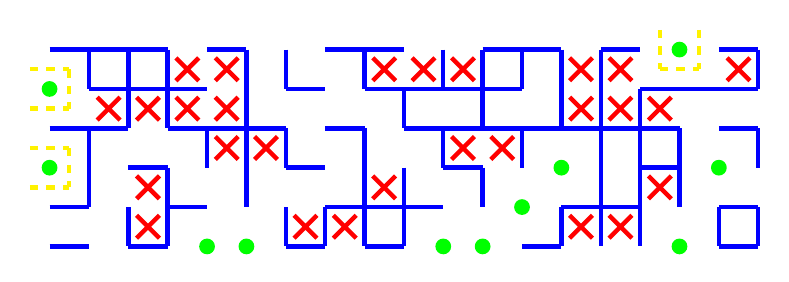
\begin{tikzpicture}[x=0.5cm, y=-0.5cm, ultra thick, blue]
% Walls
    \draw (0,0) -- (3,0);
    \draw (4,0) -- (5,0);
    \draw (7,0) -- (9,0);
    \draw (11,0) -- (13,0);
    \draw (14,0) -- (15,0);
    \draw (17,0) -- (18,0);
    \draw (1,1) -- (4,1);
    \draw (6,1) -- (7,1);
    \draw (8,1) -- (12,1);
    \draw (15,1) -- (18,1);
    \draw (0,2) -- (2,2);
    \draw (3,2) -- (6,2);
    \draw (7,2) -- (8,2);
    \draw (9,2) -- (16,2);
    \draw (17,2) -- (18,2);
    \draw (2,3) -- (3,3);
    \draw (6,3) -- (7,3);
    \draw (10,3) -- (11,3);
    \draw (15,3) -- (16,3);
    \draw (0,4) -- (1,4);
    \draw (3,4) -- (4,4);
    \draw (7,4) -- (10,4);
    \draw (13,4) -- (15,4);
    \draw (17,4) -- (18,4);
    \draw (0,5) -- (1,5);
    \draw (2,5) -- (3,5);
    \draw (6,5) -- (7,5);
    \draw (8,5) -- (9,5);
    \draw (12,5) -- (13,5);
    \draw (17,5) -- (18,5);
    \draw (1,0) -- (1,1);
    \draw (1,2) -- (1,4);
    \draw (2,0) -- (2,2);
    \draw (2,4) -- (2,5);
    \draw (3,0) -- (3,2);
    \draw (3,3) -- (3,5);
    \draw (4,2) -- (4,3);
    \draw (5,0) -- (5,4);
    \draw (6,0) -- (6,1);
    \draw (6,2) -- (6,3);
    \draw (6,4) -- (6,5);
    \draw (7,4) -- (7,5);
    \draw (8,0) -- (8,1);
    \draw (8,2) -- (8,5);
    \draw (9,1) -- (9,2);
    \draw (9,3) -- (9,5);
    \draw (10,0) -- (10,1);
    \draw (10,2) -- (10,3);
    \draw (11,0) -- (11,2);
    \draw (11,3) -- (11,4);
    \draw (12,0) -- (12,1);
    \draw (12,2) -- (12,3);
    \draw (13,0) -- (13,2);
    \draw (13,4) -- (13,5);
    \draw (14,0) -- (14,5);
    \draw (15,1) -- (15,5);
    \draw (16,2) -- (16,4);
    \draw (17,4) -- (17,5);
    \draw (18,0) -- (18,1);
    \draw (18,2) -- (18,3);
    \draw (18,4) -- (18,5);
% Pillars
    \fill[green] (16,0) circle(0.2);
    \fill[green] (0,1) circle(0.2);
    \fill[green] (0,3) circle(0.2);
    \fill[green] (13,3) circle(0.2);
    \fill[green] (17,3) circle(0.2);
    \fill[green] (12,4) circle(0.2);
    \fill[green] (4,5) circle(0.2);
    \fill[green] (5,5) circle(0.2);
    \fill[green] (10,5) circle(0.2);
    \fill[green] (11,5) circle(0.2);
    \fill[green] (16,5) circle(0.2);
% Inner points in accessible cul-de-sacs
    \node at (3.5,0.5) {};
    \node at (4.5,0.5) {};
    \node at (8.5,0.5) {};
    \node at (9.5,0.5) {};
    \node at (10.5,0.5) {};
    \node at (13.5,0.5) {};
    \node at (14.5,0.5) {};
    \node at (17.5,0.5) {};
    \node at (1.5,1.5) {};
    \node at (2.5,1.5) {};
    \node at (3.5,1.5) {};
    \node at (4.5,1.5) {};
    \node at (13.5,1.5) {};
    \node at (14.5,1.5) {};
    \node at (15.5,1.5) {};
    \node at (4.5,2.5) {};
    \node at (5.5,2.5) {};
    \node at (10.5,2.5) {};
    \node at (11.5,2.5) {};
    \node at (2.5,3.5) {};
    \node at (8.5,3.5) {};
    \node at (15.5,3.5) {};
    \node at (2.5,4.5) {};
    \node at (6.5,4.5) {};
    \node at (7.5,4.5) {};
    \node at (13.5,4.5) {};
    \node at (14.5,4.5) {};
% Entry-exit paths without intersections
    \draw[dashed, yellow] (-0.5,0.5) -- (0.5,0.5);
    \draw[dashed, yellow] (15.5,0.5) -- (16.5,0.5);
    \draw[dashed, yellow] (-0.5,1.5) -- (0.5,1.5);
    \draw[dashed, yellow] (-0.5,2.5) -- (0.5,2.5);
    \draw[dashed, yellow] (-0.5,3.5) -- (0.5,3.5);
    \draw[dashed, yellow] (0.5,0.5) -- (0.5,1.5);
    \draw[dashed, yellow] (0.5,2.5) -- (0.5,3.5);
    \draw[dashed, yellow] (15.5,-0.5) -- (15.5,0.5);
    \draw[dashed, yellow] (16.5,-0.5) -- (16.5,0.5);
\end{tikzpicture}
\end{center}
\vspace*{\fill}

\end{document}
